\newpage
\section{Цель работы}
\hspace*{\parindent}Получить опыт определения математической модели исследуемого объекта управления.
Собрать требуемый робототехнический механизм.

\section{Порядок выполнения работы}
\begin{enumerate}
	\item Соберите требуемого робота. Особое внимание при этом обратите на строение крепежного узла, соединяющего маятник с тележкой. Он должен быть представлен датчиком HiTechnic Angle Sensor (см. рис.~\ref{sensor}).
	
	Также следует учесть следующее. 
	
	При построении математической модели механической системы на используемом для этого рисунке последняя показывается в том состоянии, которому соответствуют положительные значения обобщенных координат\lefteqn.\footnote{Достаточно очевидно, что обобщенные координаты могут принимать как положительные, так и отрицательные значения. Например, в случае c нашим устройством при отклонении маятника из положения равновесия в одну сторону угол $\psi$ будет б\'oльшим нуля, в другую~--- меньшим нуля. То же можно сказать и про угол $\theta$.} Из указанной причины следует, что отмеченные на рис.~\ref{cart_in_decart} или~\ref{forces} углы $\psi$ и $\theta$ положительны. Отсюда можно сделать вывод, что отсчет данных углов у конструируемого робота должен производится аналогичным образом. 
	\item Измерьте все параметры робота, встречающиеся в его математической модели, например массу колес, длину маятника. 
	\item Постройте схему моделирования робота в Xcos. Этим будет сделана заготовка для следующей лабораторной, в которой на месте красной подписи <<$U(t)$>> будет сформировано управляющее воздействие. 
	
	При работе над ней учтите, что значения полей Initial state у интеграторов в отличие от прошлых лабораторных работ не должны быть равными нулю. В~этот раз в них следует прописать название тех переменных (в каждый блок свою), в которых будут храниться начальные условия, например psi0, dpsi0, dtheta0. В~таком случае, если надо будет, например, исследовать поведение механизма при начальном отклонении покоящегося маятника на $\pi/12 \text{ рад}$ и покоящейся тележке, необходимо будет перед моделированием дать в Scilab команду: \verb|psi0=%pi/12, dpsi0=0, dtheta0=0|. 
\end{enumerate}

\newpage
\section{Приложение А\\
Основы работы с датчиком HiTechnic Angle Sensor}
\hspace*{\parindent}HiTechnic Angle Sensor представляет из себя датчик, измеряющий разные количественные характеристики, описывающие вращение собственного <<ротора>>.
Под последним подразумевается его подвижная часть.

\begin{figure}[h]
	\noindent\centering{ 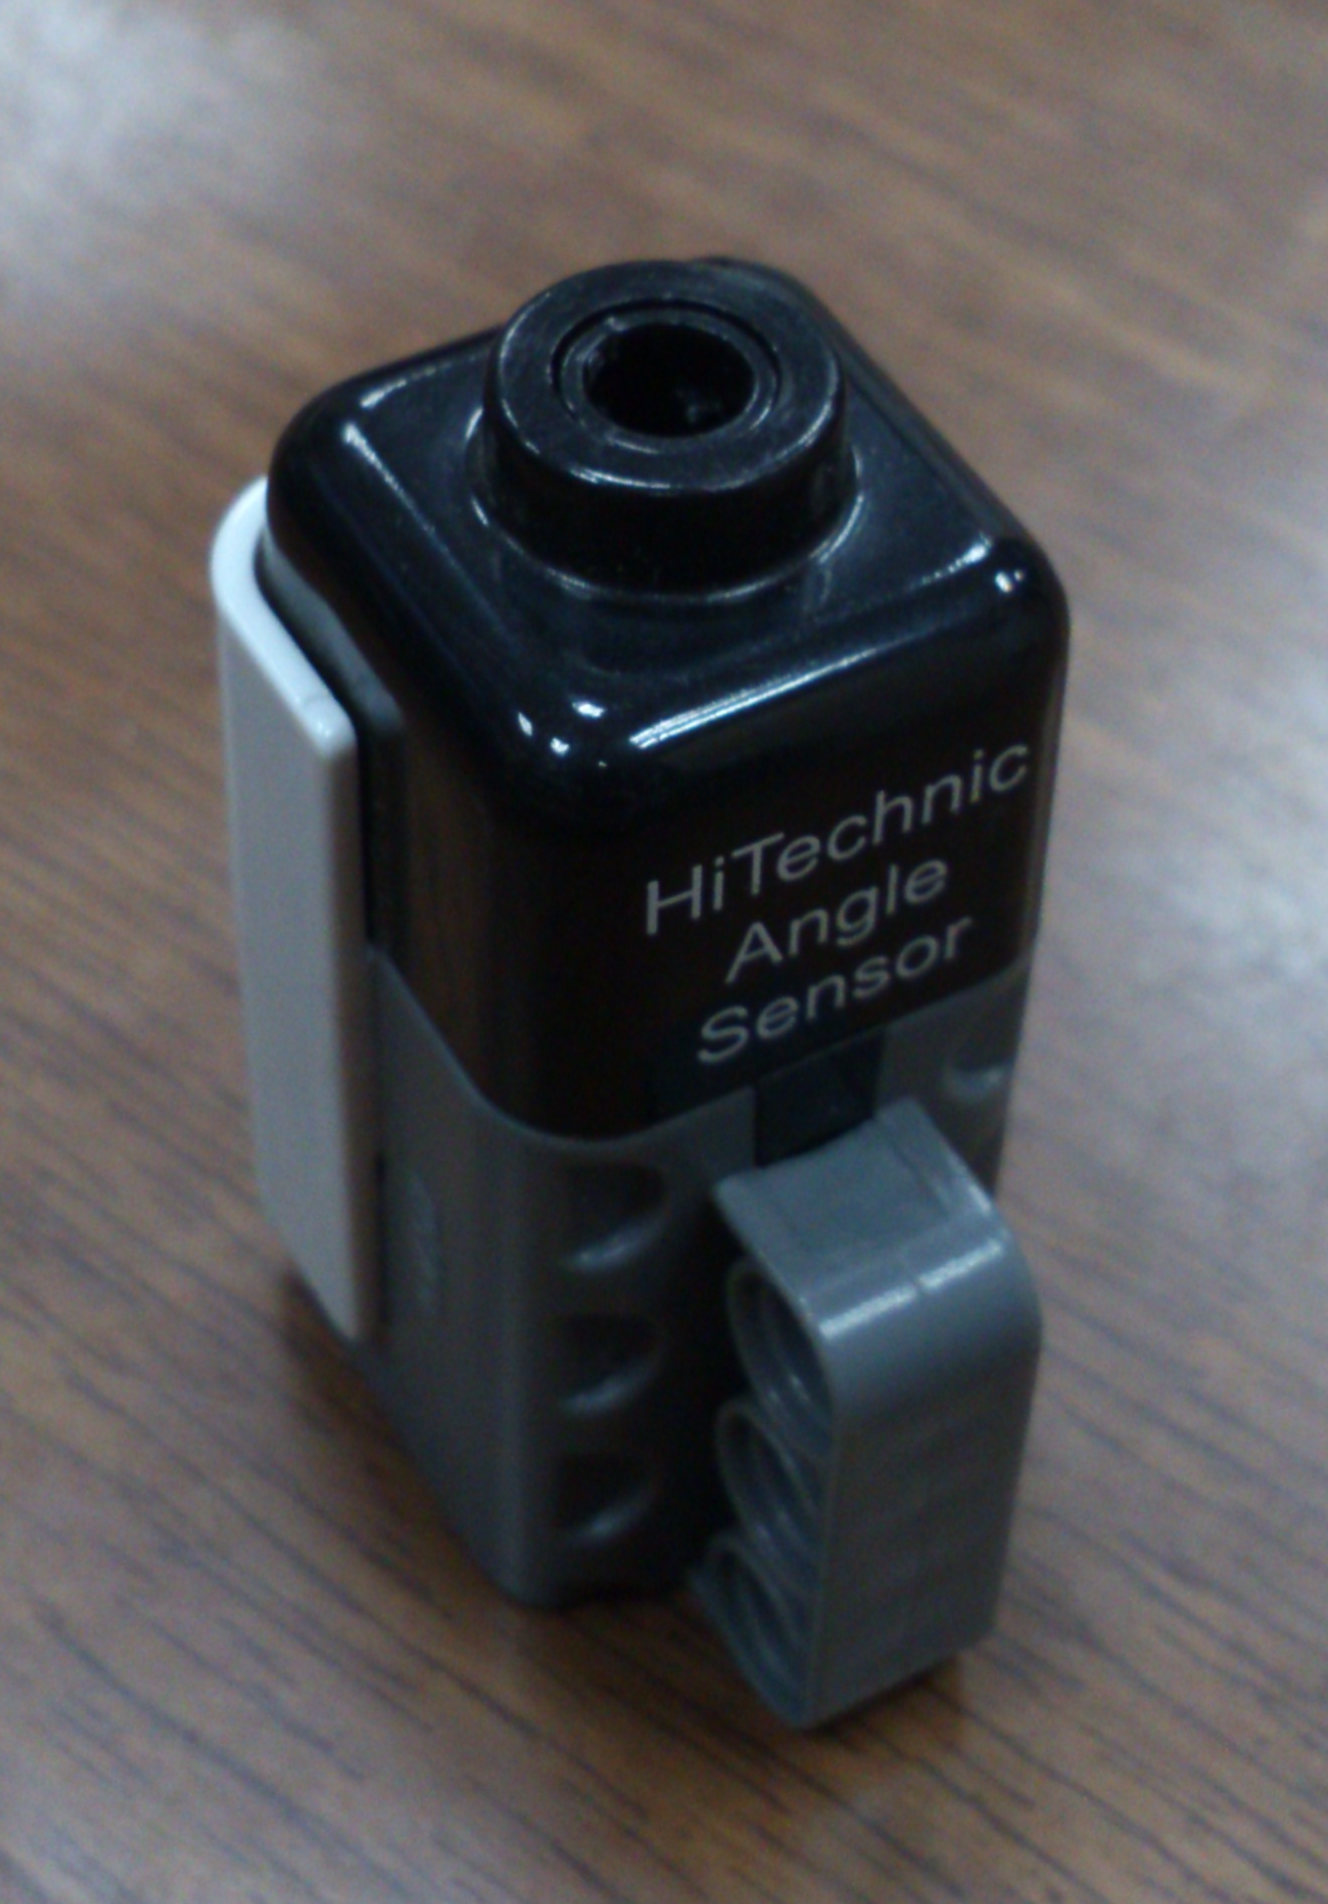
\includegraphics[scale=0.13]{sensor.png} }
	\caption{Общий вид датчика.}
	\label{sensor}
\end{figure}

Чтобы подключить этот датчик к программе, написанной на языке NXC, в нее необходимо добавить функцию \verb|SetSensorLowspeed(sensor_port)|.
Ее единственный аргумент~--- номер порта, к которому датчик подключен.

Считывание данных производится функцией \verb|ReadSensorHTAngle(sensor_port, abs_angle,| \verb|alg_angle, rpm)|.
В результате своего вызова она возвращает с датчика, подключенного в порт sensor\_port, три значения (по порядку): угловую координату (в градусах) текущего положения <<ротора>>, представляющую собой число от $0$ до $360$; угол отклонения (в градусах) от некоторого положения, представляющий из себя целое число, лежащее в диапазоне $(-2147483648;\ 2147483647)$; угловую скорость (в $\text{об}/\text{мин}$) вращения <<ротора>>~--- целое число, принадлежащее интервалу $(-1000;\ 1000)$.

В ряде случаев появляется необходимость обнулить (сбросить) текущие показание датчика.
Сделать это можно с помощью функции \verb|ResetSensorHTАngle(sensor_port, mode)|, причем значение последнего ее аргумента, являющего из себя целочисленную константу, следует принять равным макросу \verb|HTANGLE_MODE_CALIBRATE|, если надо обнулить обе величины abs\_angle и alg\_angle, а равным макросу \verb|HTANGLE_MODE_RESET|, если надо сбросить только alg\_angle.

Например, в приведенном ниже тексте некоторой программы с датчика (у которого все показания были предварительно обнулены), подключенного в порт~№2, снимаются выше указанные данные, и их значения записываются в переменные p1, p2 и p3:
\begin{verbatim}
task main(){	
    int p1, p3;
    long p2;
    ...
    SetSensorLowspeed(S2);
    ResetSensorHTАngle(S2, HTANGLE_MODE_CALIBRATE);
    ...
    ReadSensorHTAngle(S2, p1, p2, p3);
    ...
}	
\end{verbatim}     
